\documentclass[11pt, a4paper]{article}
\usepackage{pdfpages}
\usepackage{parallel}
\usepackage[T2A]{fontenc}
\usepackage{ucs}
\usepackage[utf8x]{inputenc}
\usepackage[polish,english,russian]{babel}
\usepackage{hyperref}
\usepackage{rotating}
\usepackage[inner=2cm,top=1.8cm,outer=2cm,bottom=2.3cm,nohead]{geometry}
\usepackage{listings}
\usepackage{graphicx}
\usepackage{wrapfig}
\usepackage{longtable}
\usepackage{indentfirst}
\usepackage{array}
\usepackage{tikzsymbols}
\usepackage{soul}
\usepackage[ruled,vlined]{algorithm2e}
%\counterwithout{figure}{section} 

\usepackage{url}
\makeatletter
\g@addto@macro{\UrlBreaks}{\UrlOrds}
\makeatother

\newcolumntype{P}[1]{>{\raggedright\arraybackslash}p{#1}}
\frenchspacing
\usepackage{fixltx2e} %text sub- and superscripts
\usepackage{icomma} % коскі ў матэматычным рэжыме
\PreloadUnicodePage{4}

\newcommand{\longpage}{\enlargethispage{\baselineskip}}
\newcommand{\shortpage}{\enlargethispage{-\baselineskip}}

\def\switchlang#1{\expandafter\csname switchlang#1\endcsname}
\def\switchlangbe{
\let\saverefname=\refname%
\def\refname{Літаратура}%
\def\figurename{Іл.}%
}
\def\switchlangen{
\let\saverefname=\refname%
\def\refname{References}%
\def\figurename{Fig.}%
}
\def\switchlangru{
\let\saverefname=\refname%
\let\savefigurename=\figurename%
\def\refname{Литература}%
\def\figurename{Рис.}%
}

\hyphenation{admi-ni-stra-tive}
\hyphenation{ex-pe-ri-ence}
\hyphenation{fle-xi-bi-li-ty}
\hyphenation{Py-thon}
\hyphenation{ma-the-ma-ti-cal}
\hyphenation{re-ported}
\hyphenation{imp-le-menta-tions}
\hyphenation{pro-vides}
\hyphenation{en-gi-neering}
\hyphenation{com-pa-ti-bi-li-ty}
\hyphenation{im-pos-sible}
\hyphenation{desk-top}
\hyphenation{elec-tro-nic}
\hyphenation{com-pa-ny}
\hyphenation{de-ve-lop-ment}
\hyphenation{de-ve-loping}
\hyphenation{de-ve-lop}
\hyphenation{da-ta-ba-se}
\hyphenation{plat-forms}
\hyphenation{or-ga-ni-za-tion}
\hyphenation{pro-gramming}
\hyphenation{in-stru-ments}
\hyphenation{Li-nux}
\hyphenation{sour-ce}
\hyphenation{en-vi-ron-ment}
\hyphenation{Te-le-pathy}
\hyphenation{Li-nux-ov-ka}
\hyphenation{Open-BSD}
\hyphenation{Free-BSD}
\hyphenation{men-ti-on-ed}
\hyphenation{app-li-ca-tion}

\def\progref!#1!{\texttt{#1}}
\renewcommand{\arraystretch}{2} %Іначай формулы ў матрыцы зліпаюцца з лініямі
\usepackage{array}

\def\interview #1 (#2), #3, #4, #5\par{

\section[#1, #3, #4]{#1 -- #3, #4}
\def\qname{LVEE}
\def\aname{#1}
\def\q ##1\par{{\noindent \bf \qname: ##1 }\par}
\def\a{{\noindent \bf \aname: } \def\qname{L}\def\aname{#2}}
}

\def\interview* #1 (#2), #3, #4, #5\par{

\section*{#1\\{\small\rm #3, #4. #5}}
\ifx\ParallelWhichBox\undefined%
    \addcontentsline{toc}{section}{#1, #3, #4}%
\else%
\ifnum\ParallelWhichBox=0%
    \addcontentsline{toc}{section}{#1, #3, #4}%
\fi\fi%

\def\qname{LVEE}
\def\aname{#1}
\def\q ##1\par{{\noindent \bf \qname: ##1 }\par}
\def\a{{\noindent \bf \aname: } \def\qname{L}\def\aname{#2}}
}

\newcommand{\interviewfooter}[1]{
\vskip 1em
\noindent \textit{#1}
}


\begin{document}

\title{1990 "--- Трекбол Kraft TopTrak}
\date{}
\maketitle

Трекбол TopTrak имеет средние размеры и корпус с закруглёнными углами (рис. \ref{fig:TopTrakPic}, \ref{fig:TopTrakTopAndBottom}).

\begin{figure}[h]
    \centering
    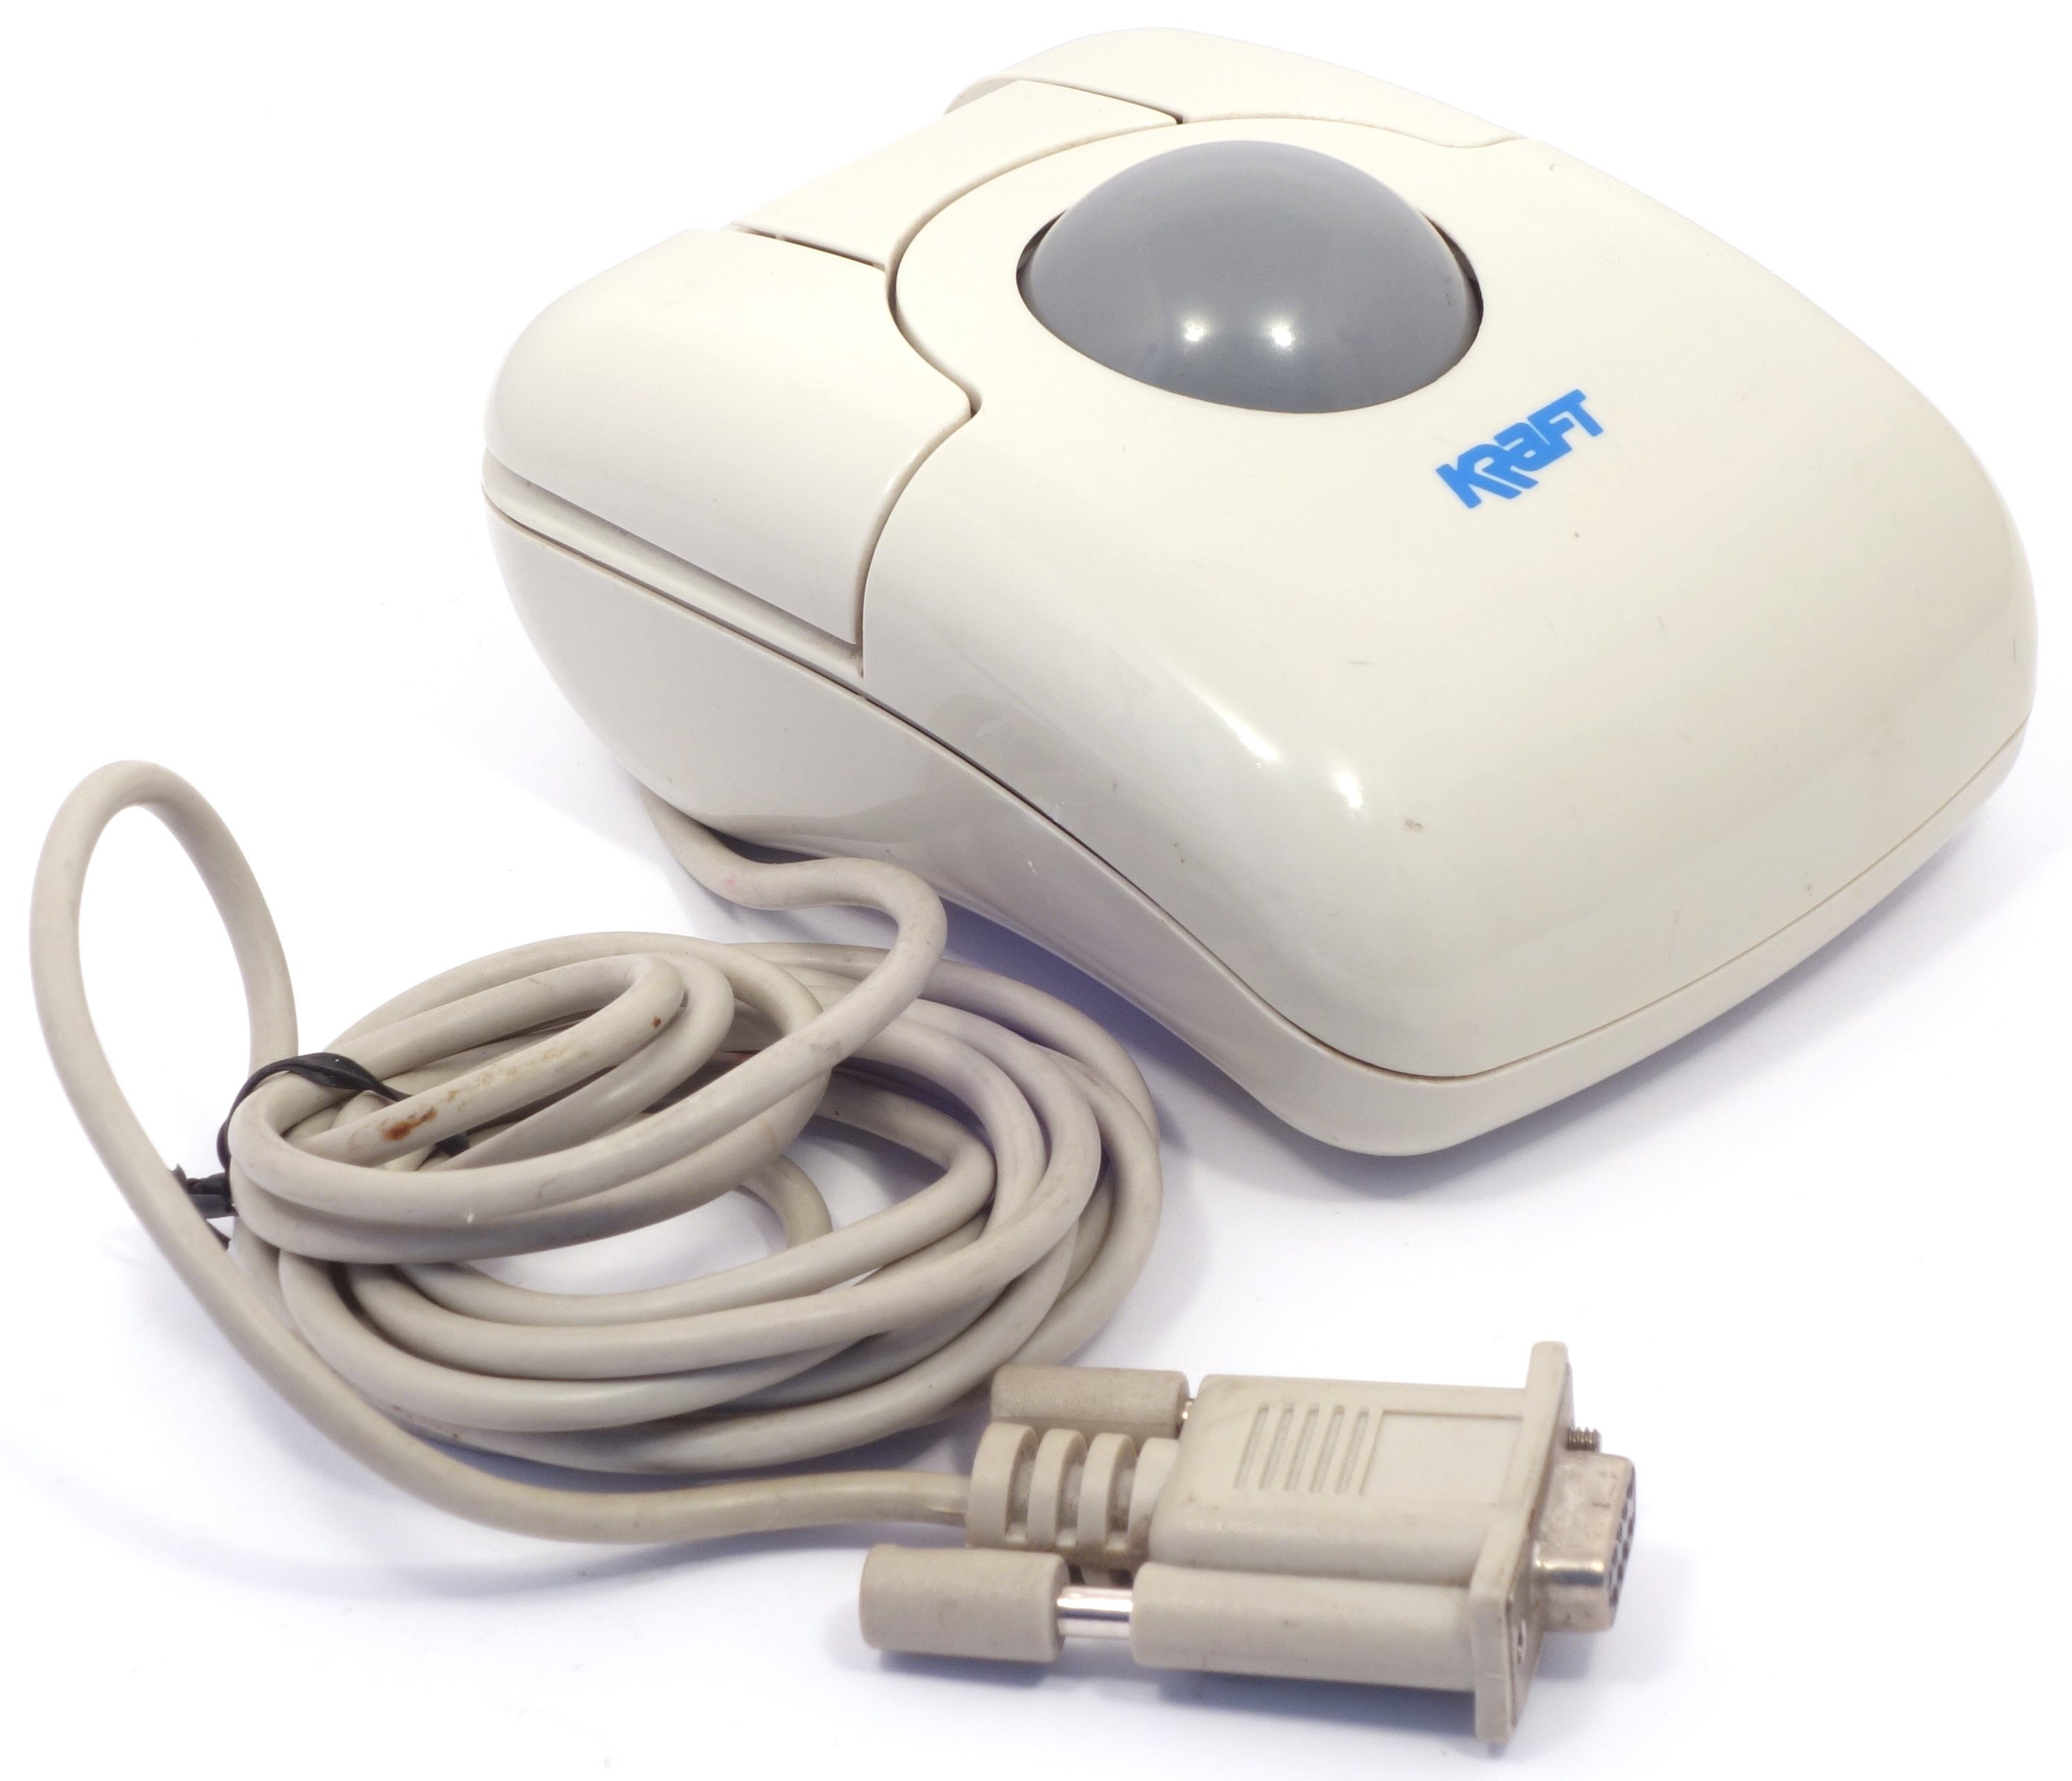
\includegraphics[scale=0.45]{1990_kraft_toptrack/pic_60.jpg}
    \caption{Изображение мыши Kraft TopTrak}
    \label{fig:TopTrakPic}
\end{figure}

Устройство снабжено кабелем длиной 2.5 м, что заметно больше типового расстояния между пользователем и системным блоком. Трекбол имеет последовательный интерфейс сопряжения с компьютером.

\begin{figure}[h]
    \centering
    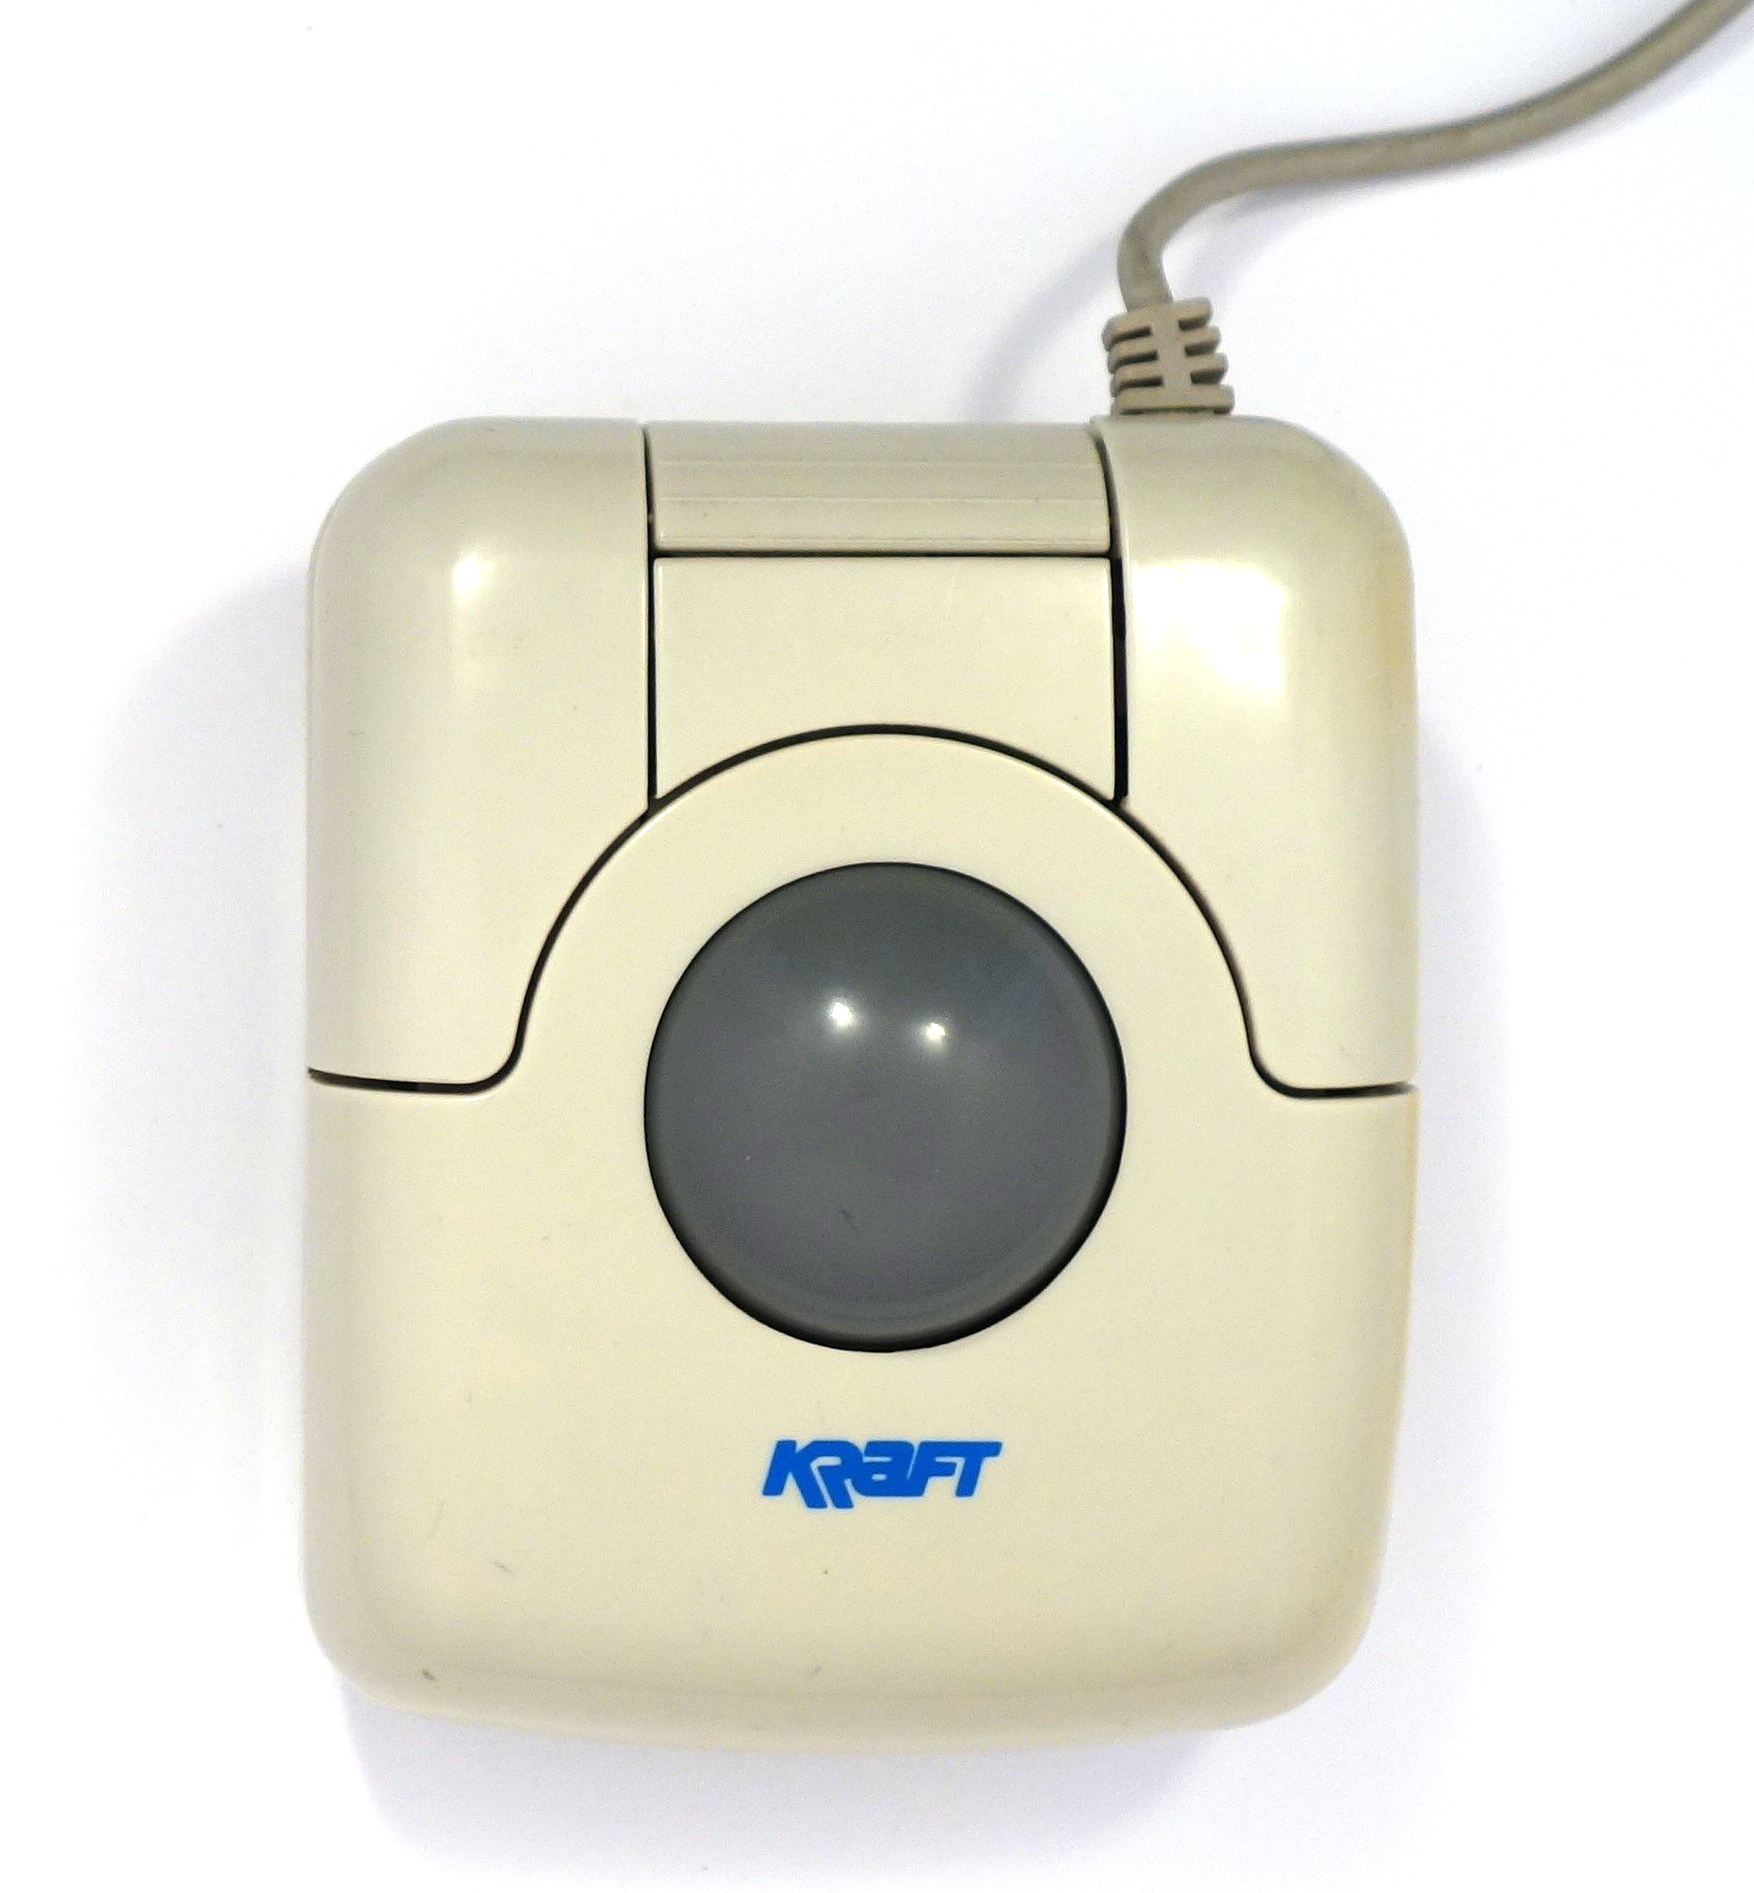
\includegraphics[scale=0.4]{1990_kraft_toptrack/2.9_60.jpg}
    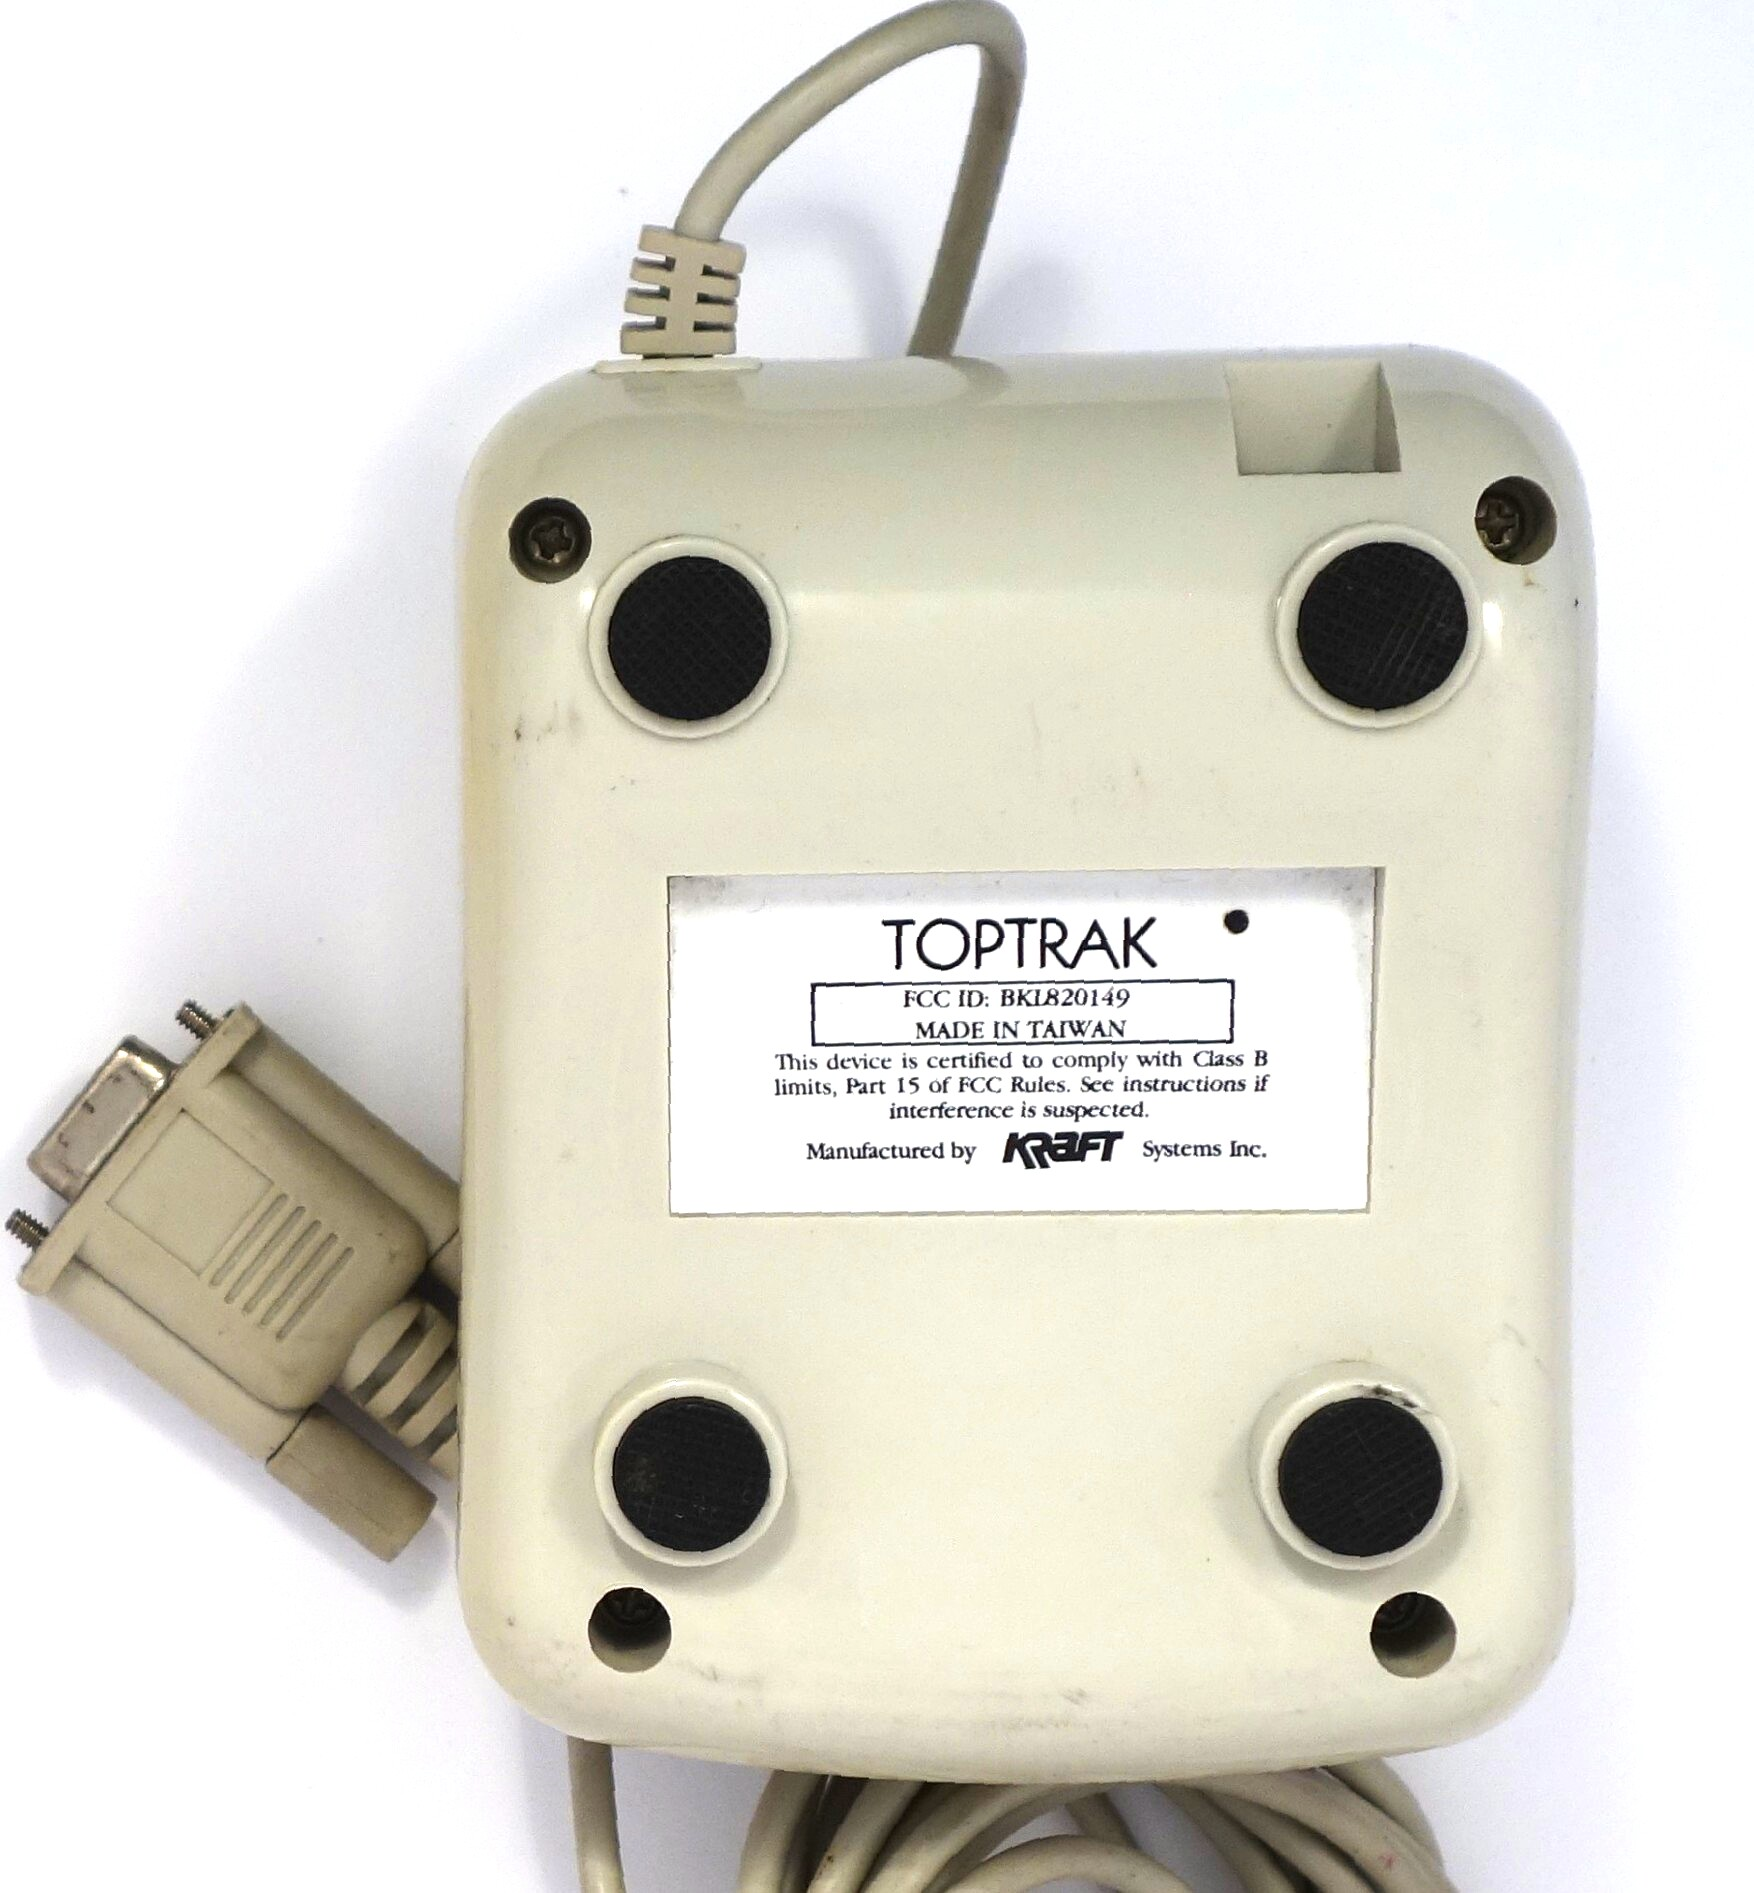
\includegraphics[scale=0.4]{1990_kraft_toptrack/2.10_60.jpg}
    \caption{TopTrak, вид сверху и снизу}
    \label{fig:TopTrakTopAndBottom}
\end{figure}

Дополнительно в комплекте с трекболом идёт стальная ножная педаль (рис. \ref{fig:TopTrakPedal}), которая служит альтернативой левой кнопке мыши, имеет еще один аналогичный кабель и добавляет дополнительные полкилограмма веса устройству \cite{mouses}.

\begin{figure}[h]
    \centering
    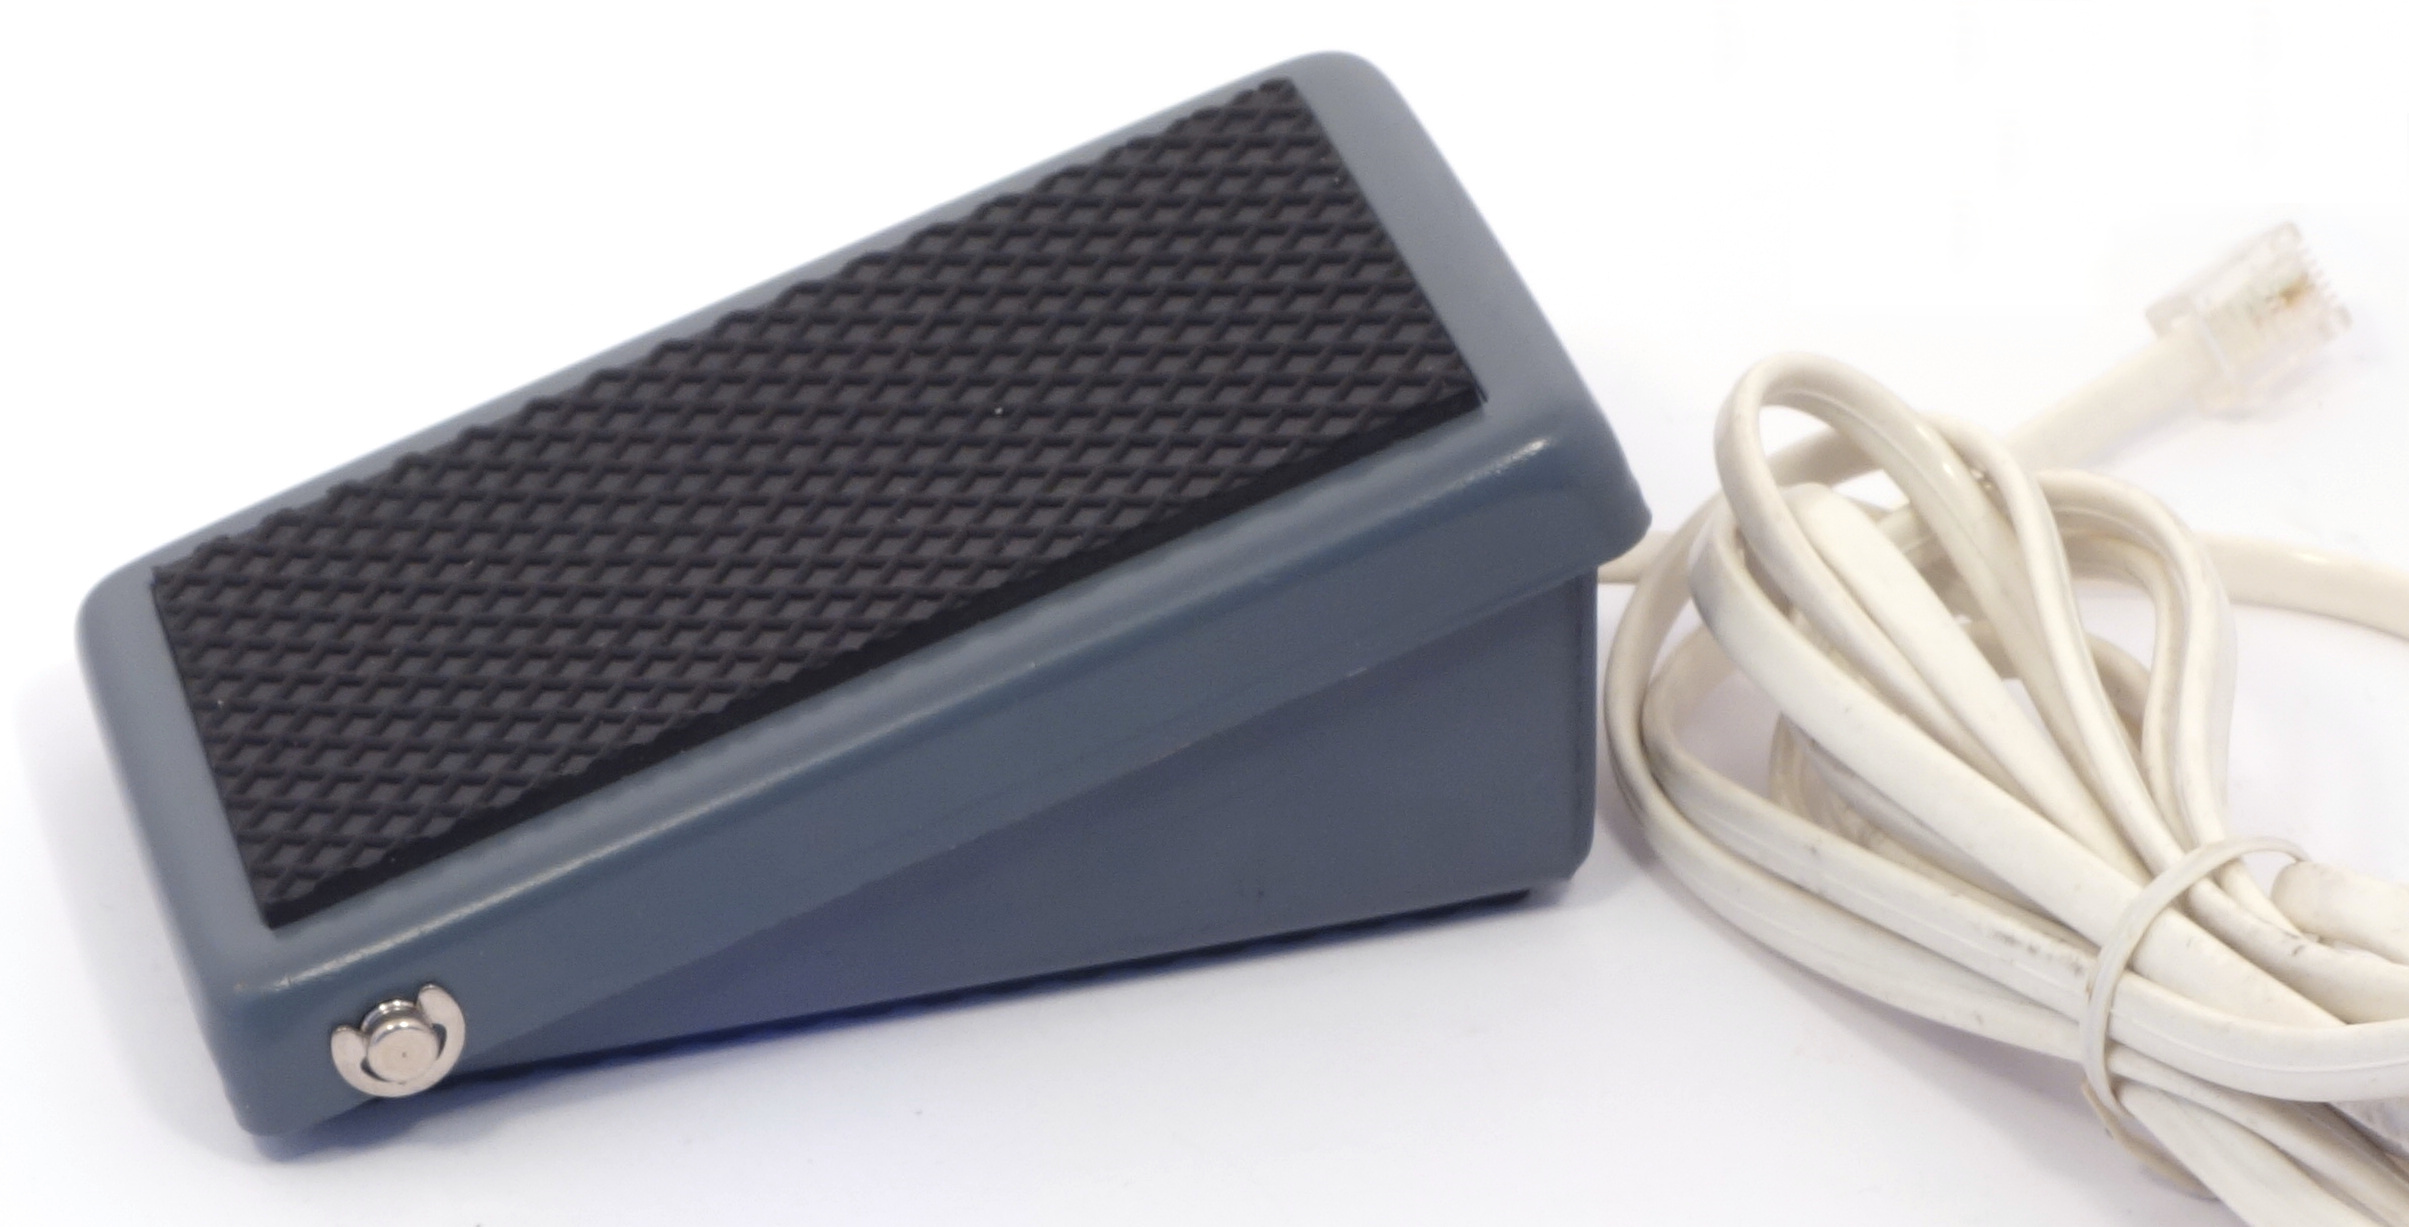
\includegraphics[scale=0.45]{1990_kraft_toptrack/pedal_30.jpg}
    \caption{Изображение педали для мыши TopTrak}
    \label{fig:TopTrakPedal}
\end{figure}

%\begin{figure}[h]
%    \centering
%    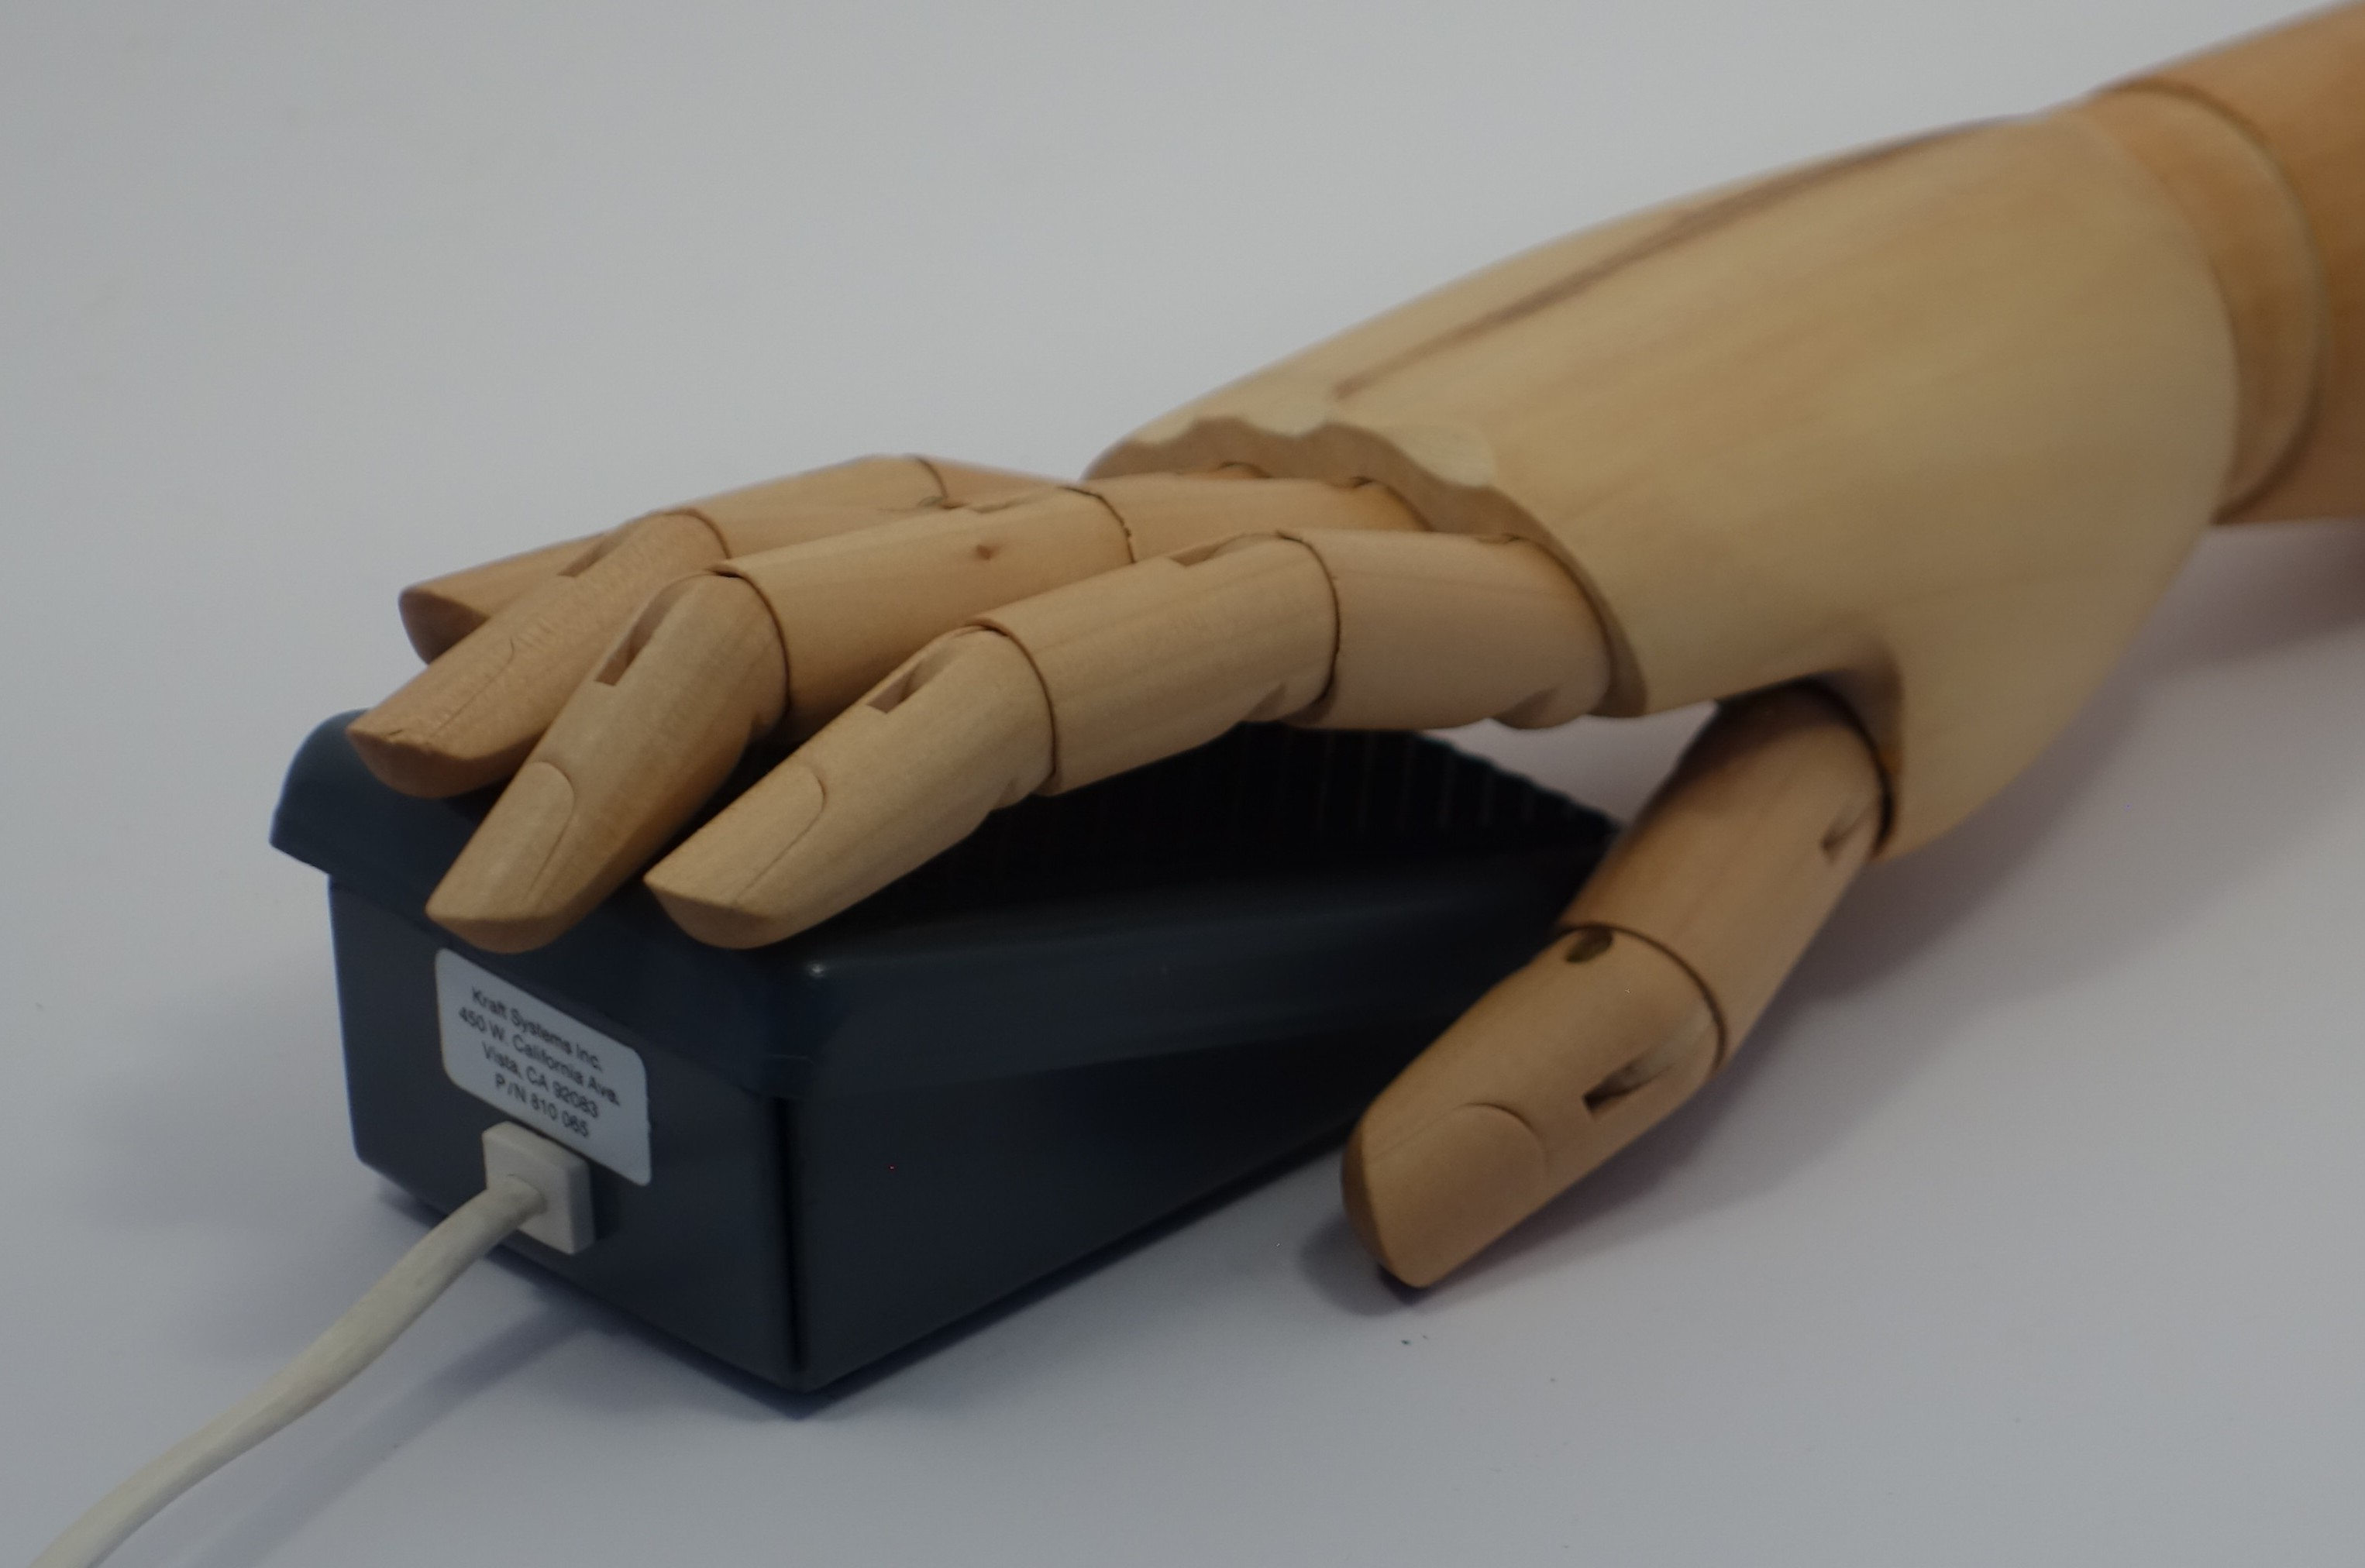
\includegraphics[scale=0.4]{1990_kraft_toptrack/2.8.jpg}
%    \caption{Изображение педали для мыши TopTrak с моделью руки человека}
%    \label{fig:TopTrakPedalHand}
%\end{figure}

Kraft TopTrak является достаточно компактным устройством (рис. \ref{fig:TopTrakSize}), в особенности в сравнении с предыдущей моделью трекбола Kraft, выпущенной в 1989 году ~--- существенно большей по размеру, имевшей подчёркнуто угловатый корпус, и комплектовавшейся в точности такой же педалью.

\begin{figure}[h]
    \centering
    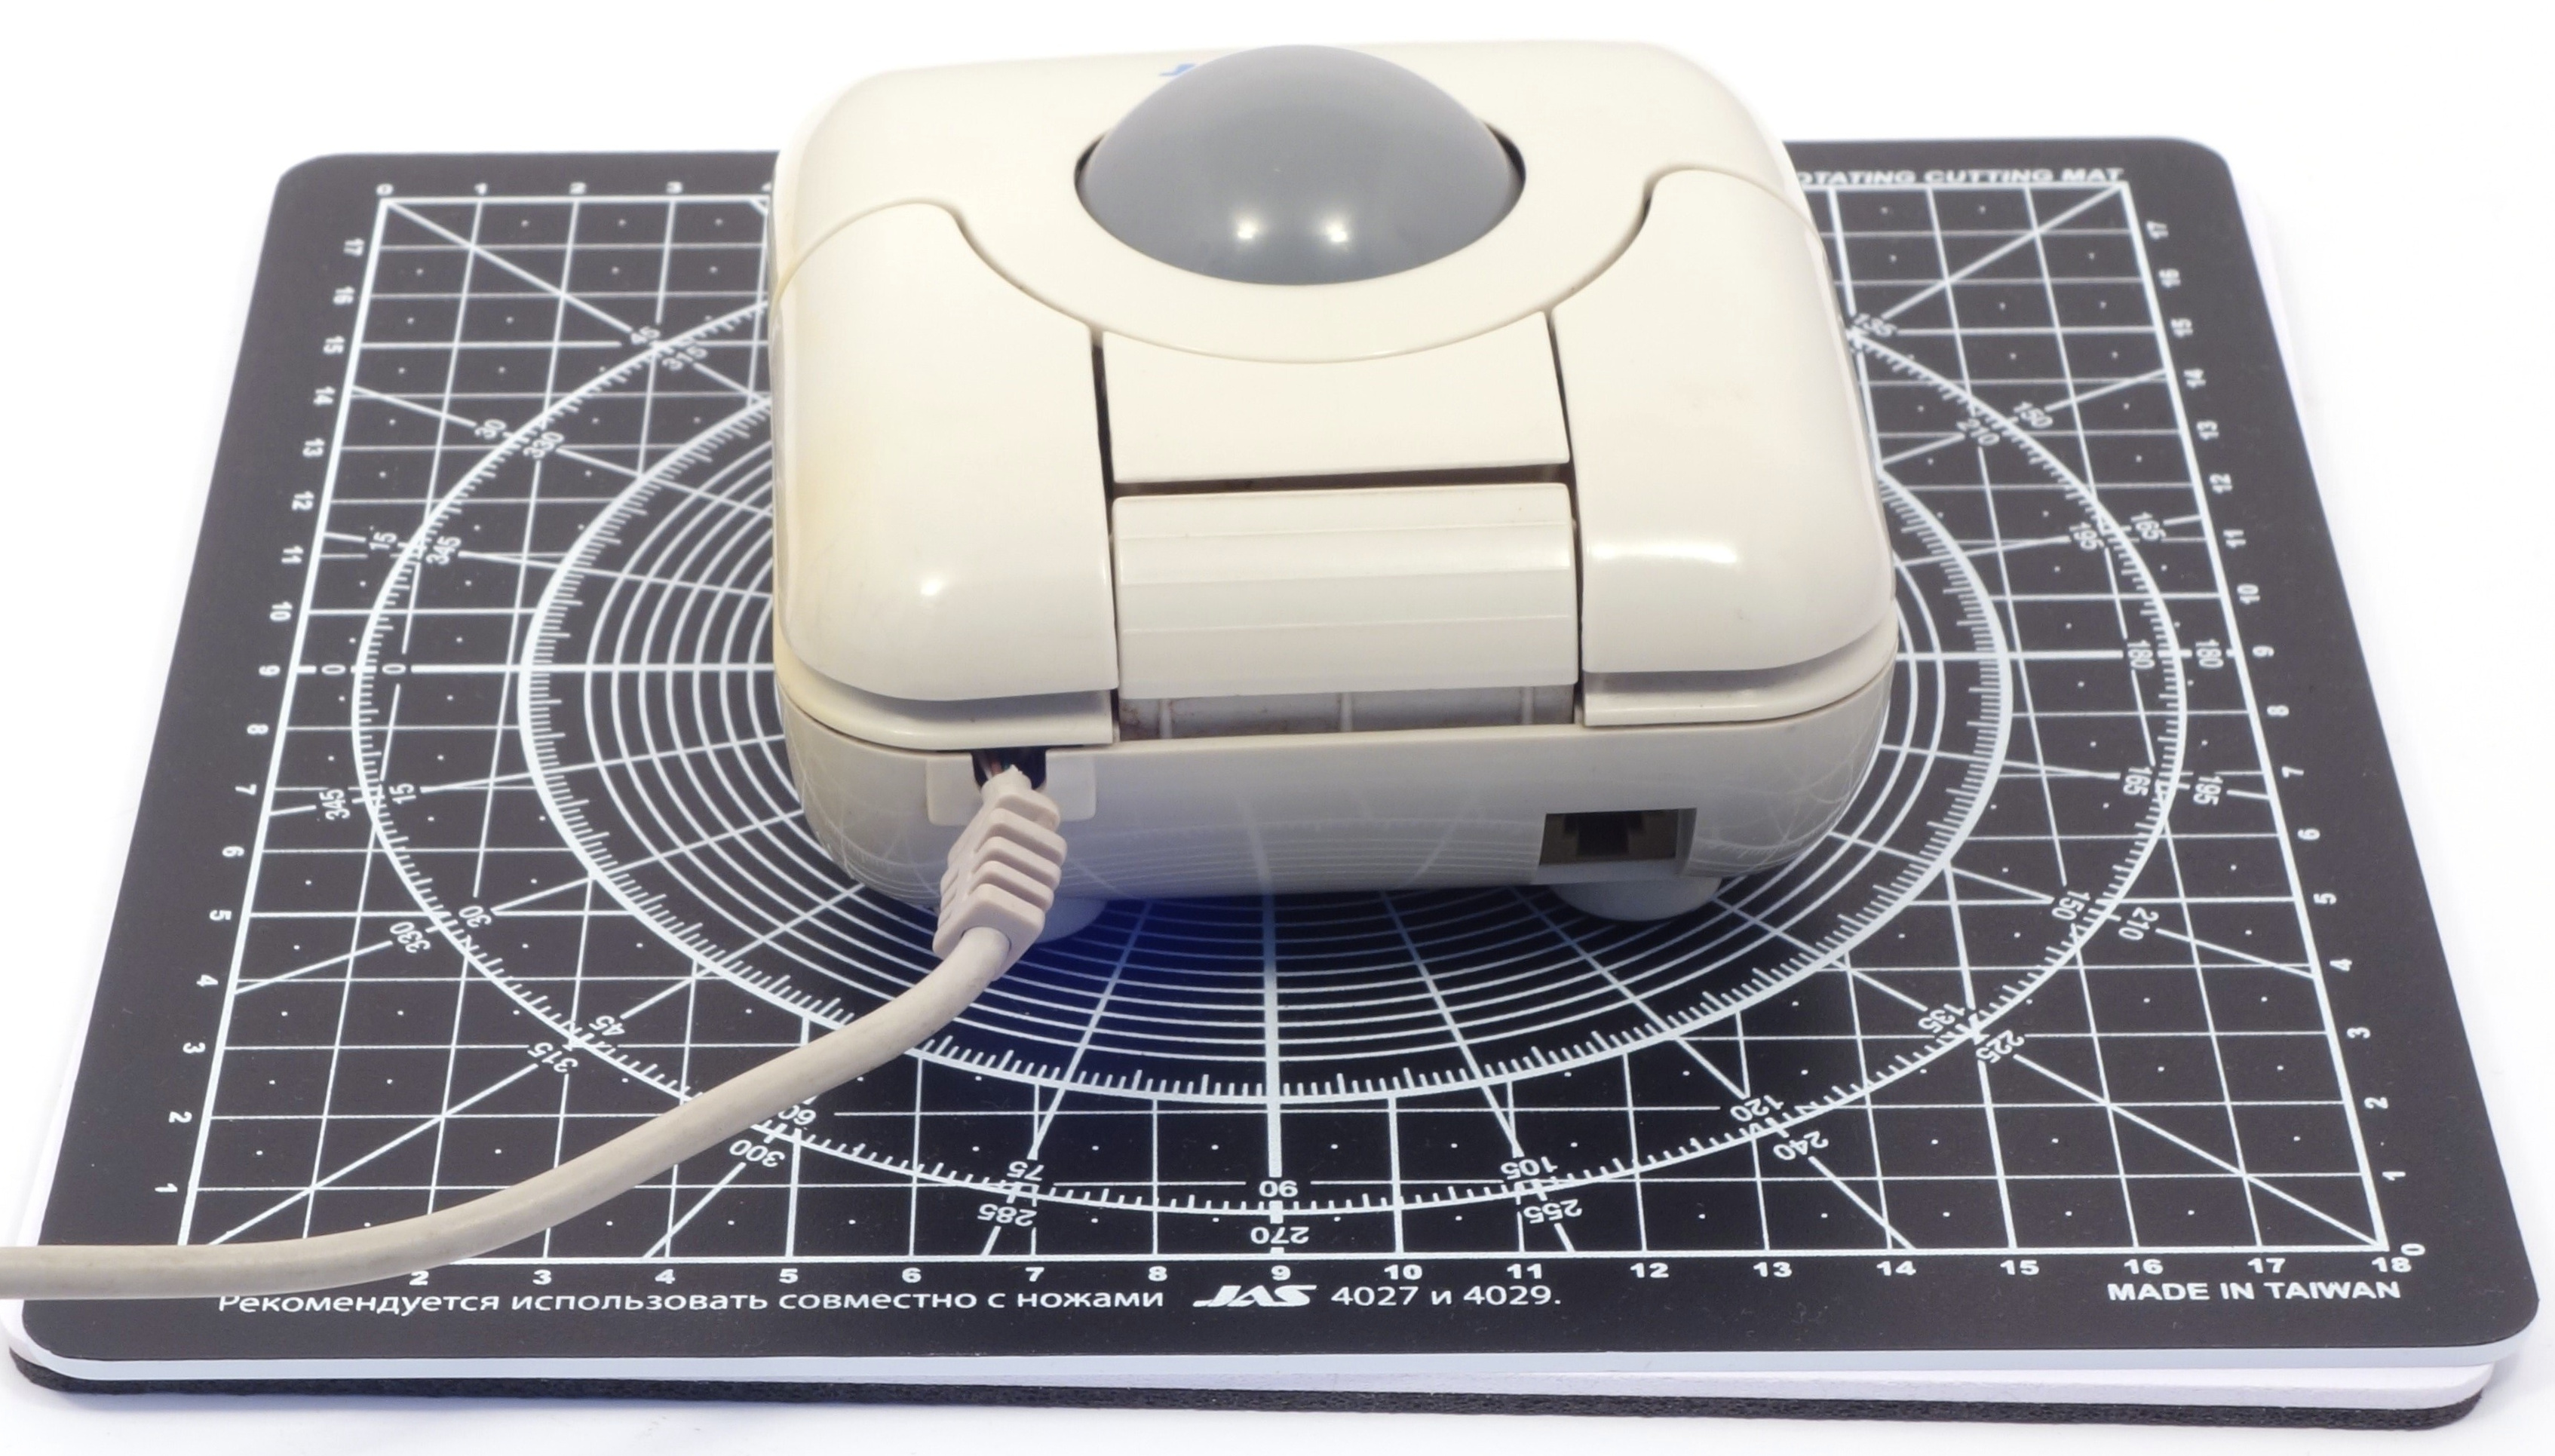
\includegraphics[scale=0.35]{1990_kraft_toptrack/2.6_30.jpg}
    \caption{Изображение TopTrak на размерном коврике с шагом сетки 1~см}
    \label{fig:TopTrakSize}
\end{figure}


Код FCC ID, присутствующий на корпусе TopTrak (рис. \ref{fig:TopTrakTopAndBottom}), показывает, что трекбол был разработан американской компанией Kraft Systems в 1990 году, всего через год после выхода предыдущей модели.

В плане эргономики TopTrak можно назвать существенным шагом вперед. Обтекаемая
форма корпуса, а также большие левая и правая кнопки, которые полностью занимают
верхние углы, обеспечивают достаточно удобное положение ладони (рис. \ref{fig:TopTrakHand}).


\begin{figure}[h]
    \centering
    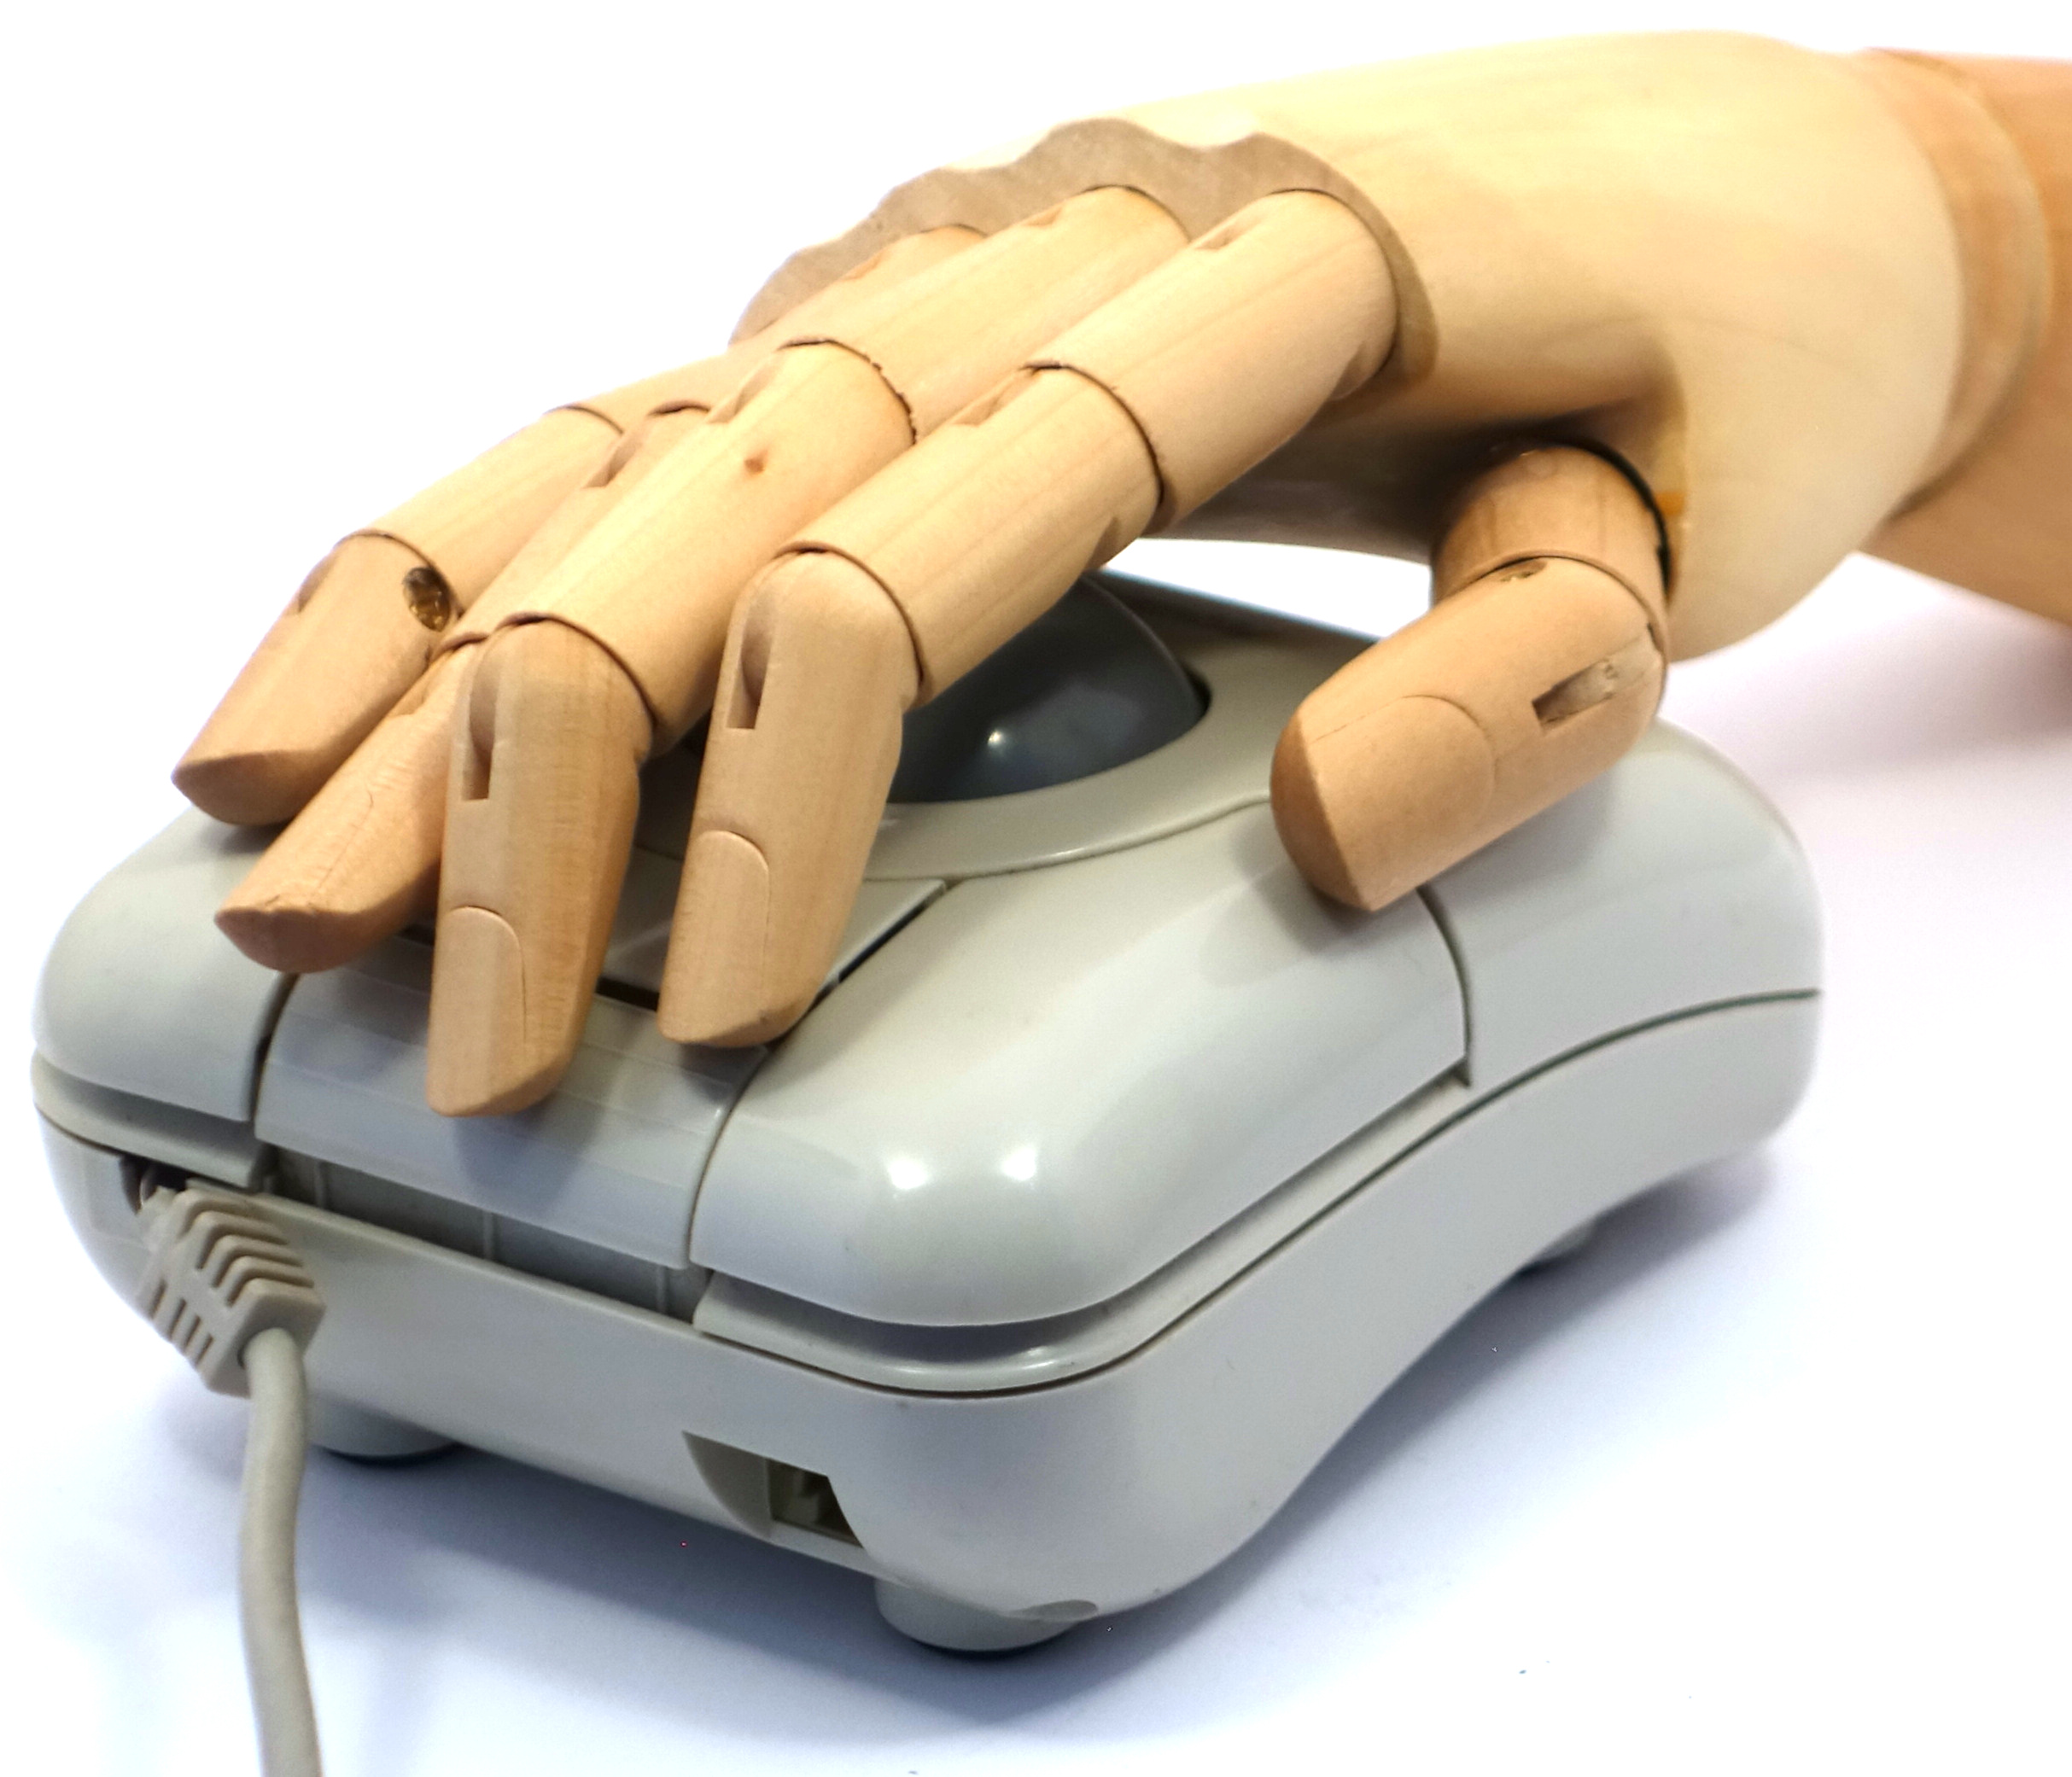
\includegraphics[scale=0.45]{1990_kraft_toptrack/hand_60.jpg}
    \caption{Изображение TopTrak с моделью руки человека}
    \label{fig:TopTrakHand}
\end{figure}


%\begin{figure}[htpb]
%    \centering
%    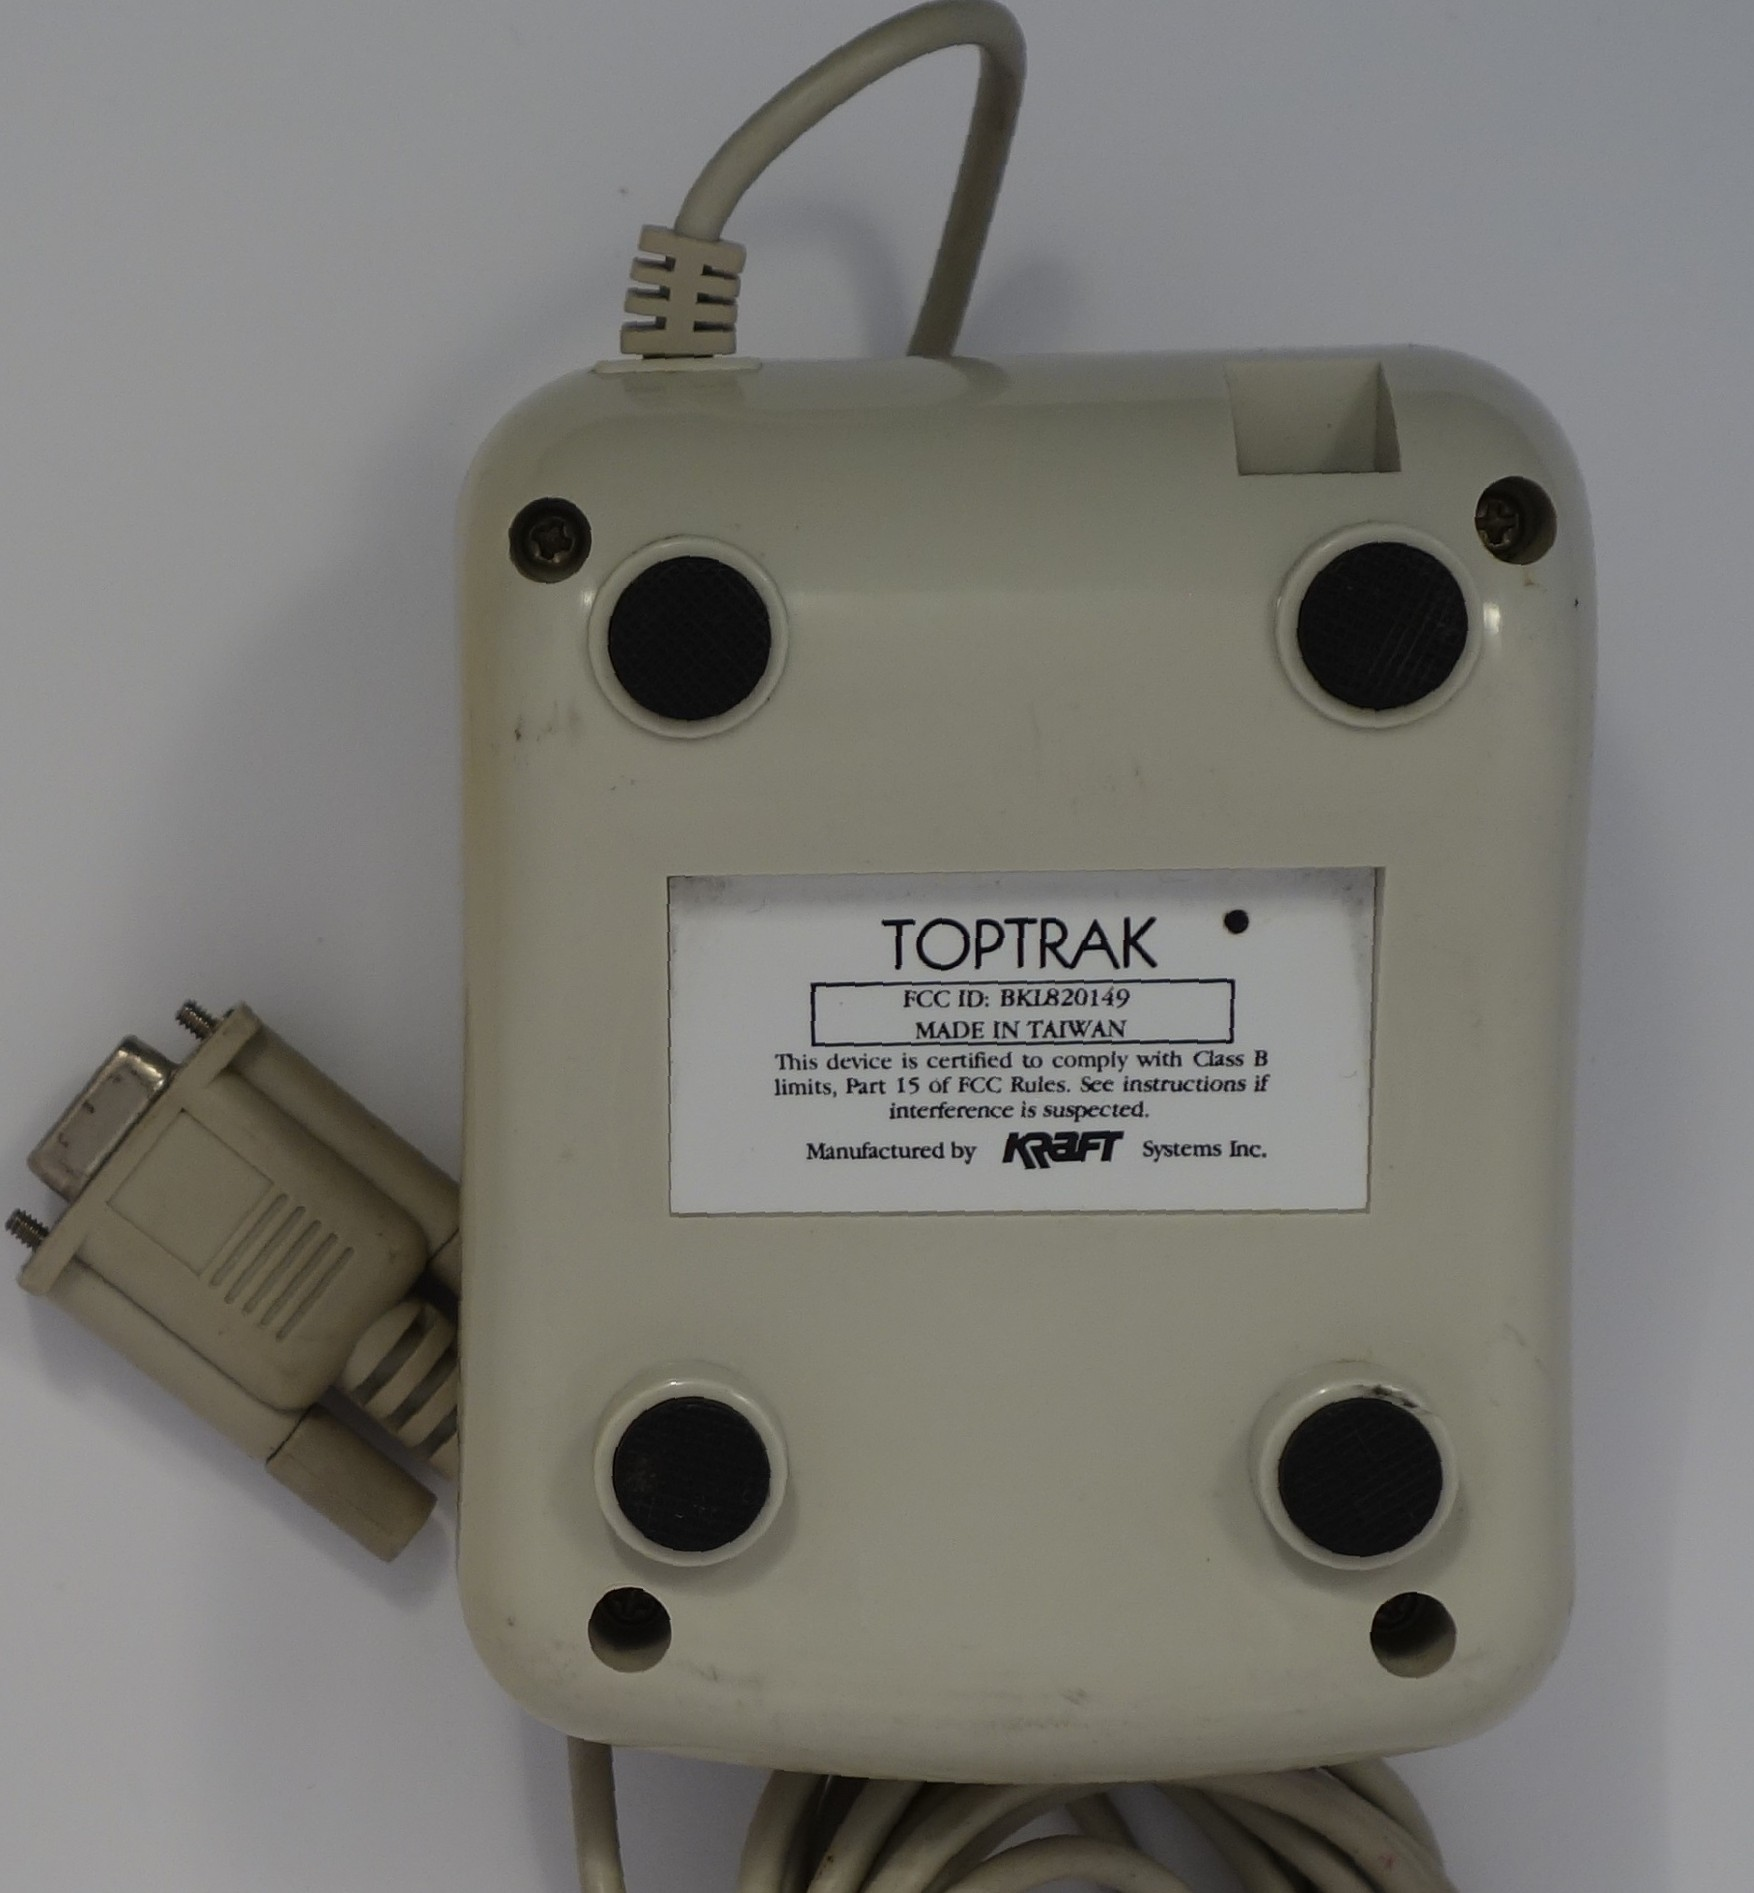
\includegraphics[scale=0.4]{1990_kraft_toptrack/2.10.jpg}
%    \caption{TopTrak, вид снизу}
%    \label{fig:TopTrakBottom}
%\end{figure}

Изучение разобранного трекбола (рис. \ref{fig:TopTrakInside}) показывает, что он выполнен по стандартной оптомеханической схеме, а массивные металлические ролики с подшипниками качения показывают, что трекбол был задуман как достаточно долговечное устройство, не относящееся к нижнему ценовому диапазону.

\begin{figure}[h]
    \centering
    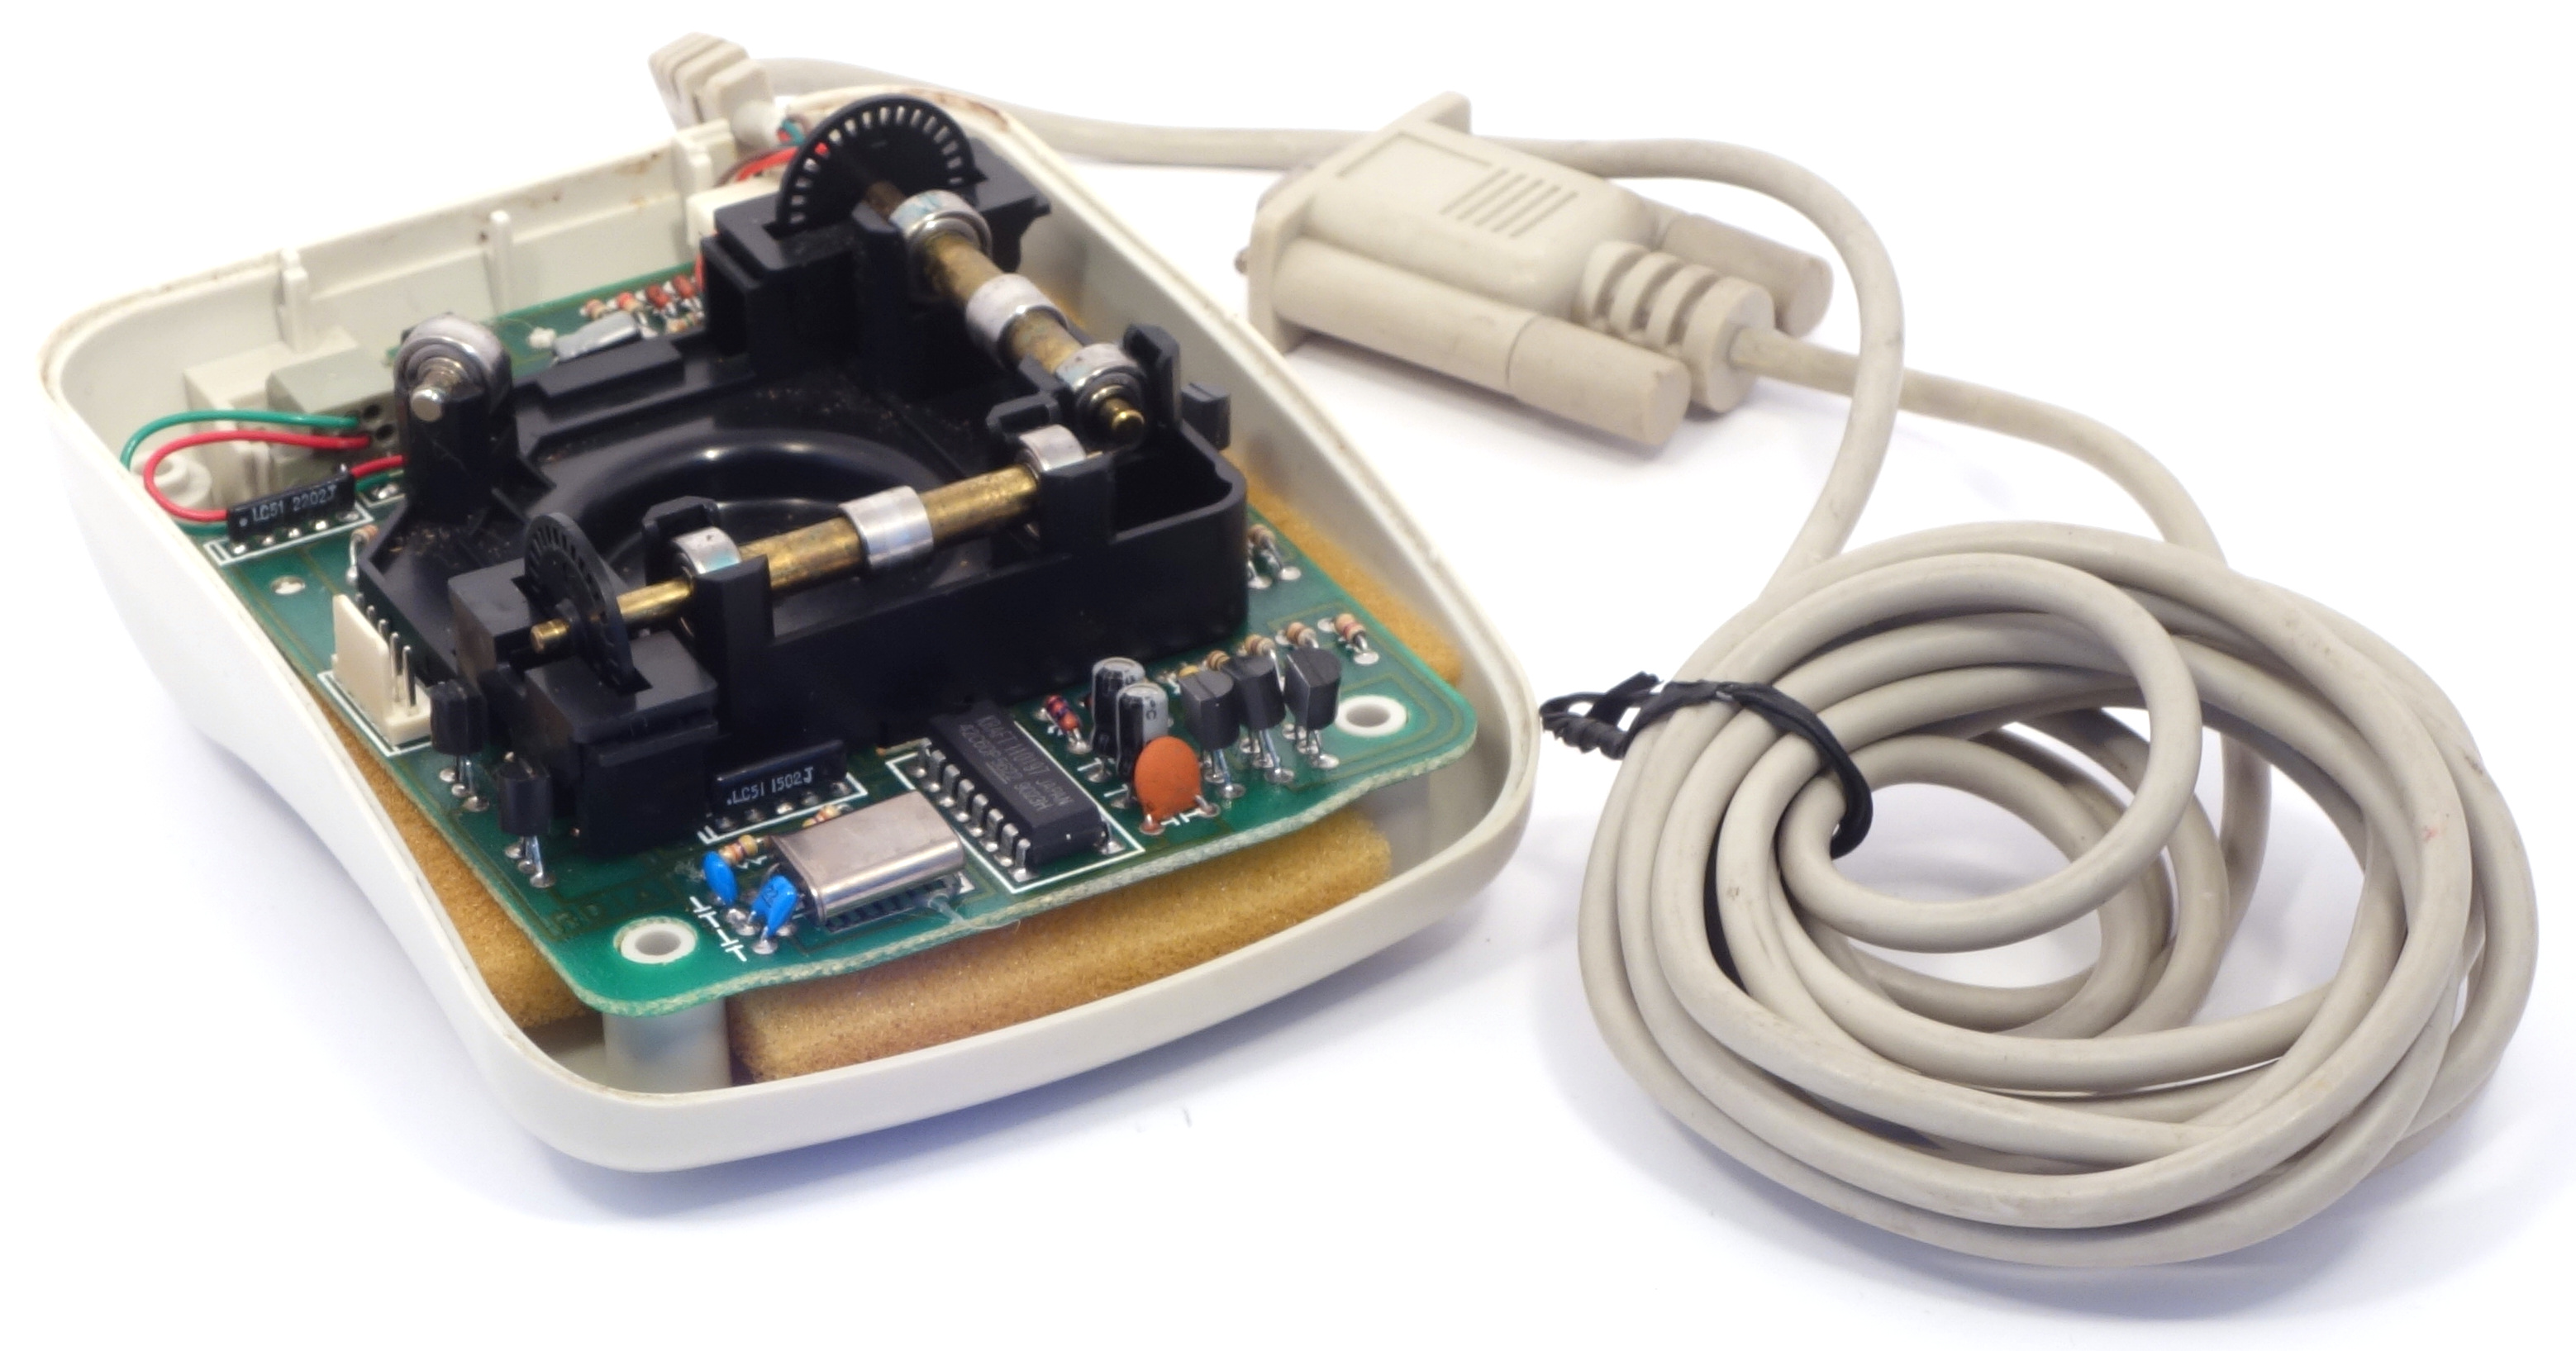
\includegraphics[scale=0.7]{1990_kraft_toptrack/inside_60.jpg}
    \caption{TopTrak изнутри}
    \label{fig:TopTrakInside}
\end{figure}

\begin{thebibliography}{9}
\bibitem {mouses} Berlin E. TopTrak // PC Magazine. October 15, 1991. p. 126-127 \url{https://books.google.by/books?id=tSLe3yMjc-AC&lpg=PP1&pg=PT123#v=onepage&q&f=false}
\end{thebibliography}
\end{document}
